\documentclass{article}
\usepackage{amsmath}
\usepackage{hyperref}
\usepackage{graphicx}
\usepackage{float}
\usepackage[a4paper, margin=1in]{geometry}
\begin{document}

% ROS 2 Robotics Training Module: Navigation and Localization with RTAB-Map

% Introduction

\section*{Modul Pelatihan Teaching Factory Programming: Navigasi dan Lokalisasi dengan RTAB-Map}
Program pelatihan ini dirancang untuk mahasiswa yang sudah memiliki pengetahuan dasar tentang ROS2.
Fokus pelatihan adalah pada navigasi, lokalisasi, navigasi waypoint, dan pengendalian misi menggunakan state machine.
Pelatihan ini menggunakan simulasi TurtleBot dan RTAB-Map.

% Module 1
\section{Modul 1: Setup \& Installasi}

\subsection{Konfigurasi Environment}
\begin{itemize}
  \item Install ROS 2 Humble
        lakukan installasi menggunakan \href{https://docs.ros.org/en/humble/Installation/Ubuntu-Install-Debs.html}{\textbf{panduan instalasi Debian}}
  \item Install TurtleBot3 packages menggunakan \href{https://emanual.robotis.com/docs/en/platform/turtlebot3/quick-start/#installing-turtlebot3-packages}{\textbf{panduan instalasi TurtleBot3}}
  \item Install Gazebo dengan \texttt{sudo apt install ros-humble-desktop}
  \item Install RViz2 dengan \texttt{sudo apt install ros-humble-rviz2}
  \item Install RTAB-Map dengan \texttt{sudo apt install ros-humble-rtabmap-ros}
  \item Install Navigation2 dengan \texttt{sudo apt install ros-humble-navigation2 ros-humble-nav2-bringup}
\end{itemize}

\subsection{Menjalankan Simulasi}
Setelah semua paket terinstal, jalankan simulasi TurtleBot3 Waffle Pi di Gazebo dengan environment \texttt{house}:
\begin{verbatim}
export TURTLEBOT3_MODEL=waffle_pi
ros2 launch turtlebot3_gazebo turtlebot3_house.launch.py
\end{verbatim}

\subsection{Teleoperation}
Buka terminal lain untuk menjalankan teleop:
\begin{verbatim}
ros2 run turtlebot3_teleop teleop_keyboard
\end{verbatim}

\subsection{RViz2}
Buka RViz2 untuk melihat topik yang dipublish dan TF yang dimiliki robot:
\begin{verbatim}
rviz2
\end{verbatim}
Atur Fixed Frame ke \texttt{odom}.
Tambahkan display untuk \texttt{LaserScan}, dan \texttt{TF}.
Sehingga akan muncul tampilan seperti berikut:
\begin{figure}[H]
  \centering
  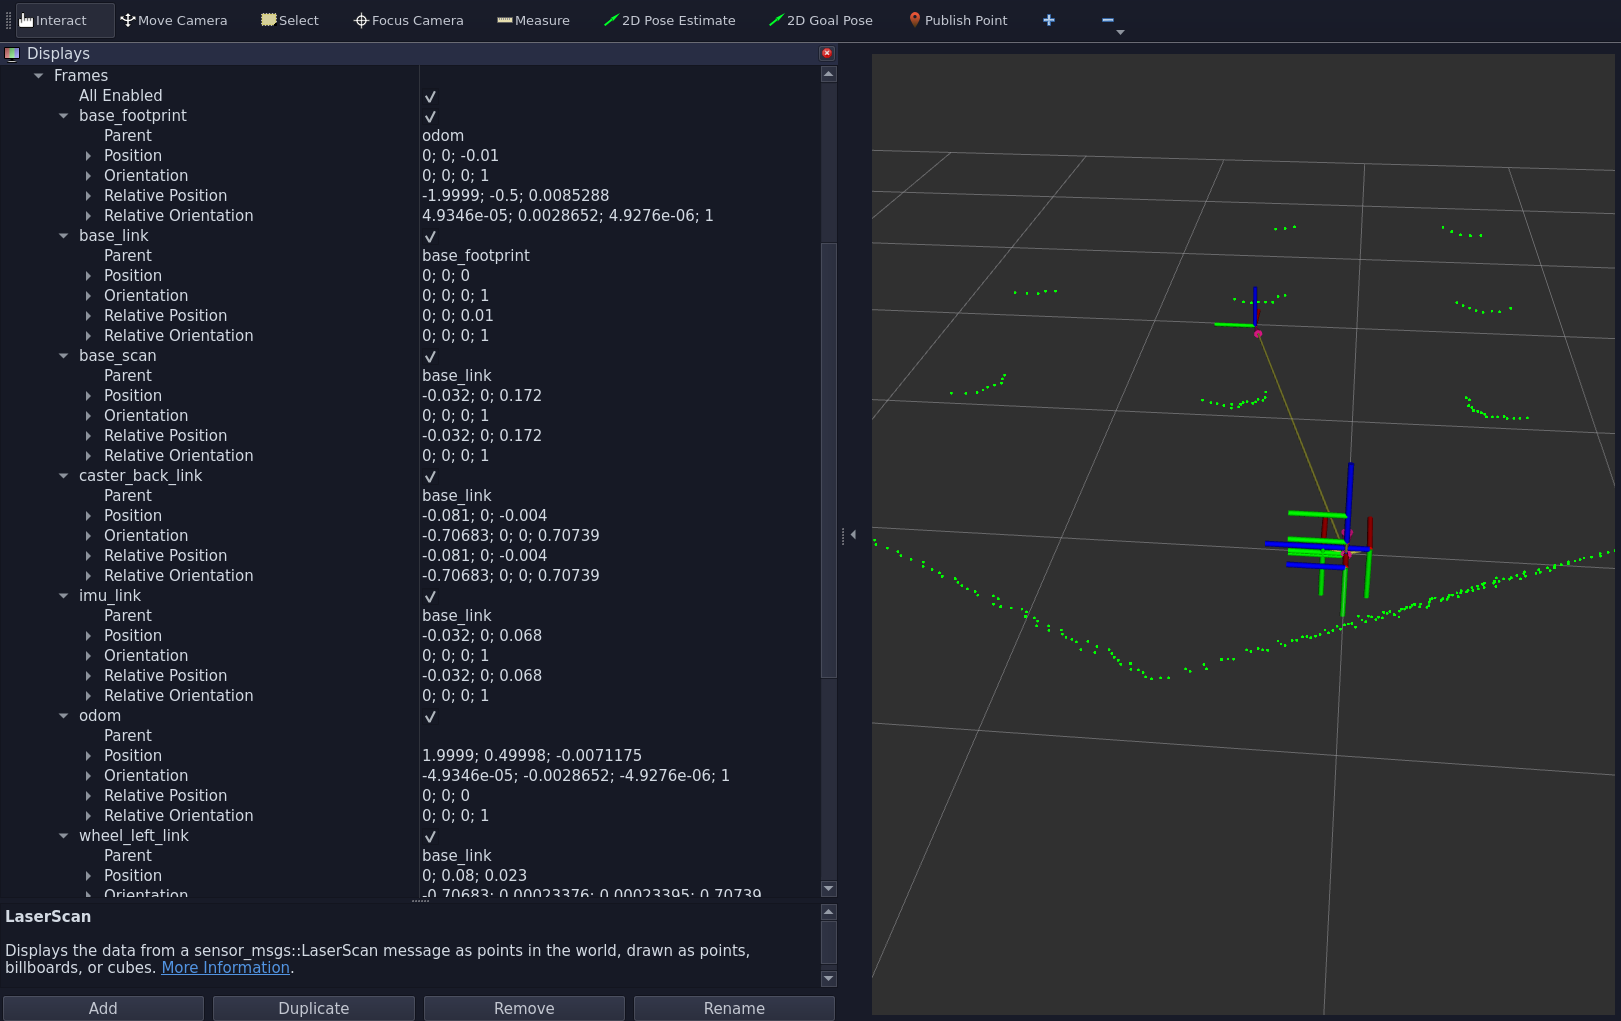
\includegraphics[width=1\textwidth]{rviz2.png}
  \caption{Contoh tampilan RViz2}
\end{figure}

Pada sidebar ditunjukkan TF yang dimiliki robot:
\begin{itemize}
  \item \texttt{odom}: frame odometri, bergerak relatif terhadap \texttt{base\_link}
  \item \texttt{base\_footprint}: frame footprint robot (sejajar dengan ground plane 2D)
  \item \texttt{base\_link}: frame utama robot (dapat mengalami translasi dan orientasi)
  \item \texttt{caster\_back\_link}: frame caster back (free wheel)
  \item \texttt{imu\_link}: frame IMU
  \item \texttt{base\_scan}: frame laser scan
  \item \texttt{wheel\_left\_link}: frame roda kiri
  \item \texttt{wheel\_right\_link}: frame roda kanan
  \item \texttt{camera\_link}: frame dasar kamera (body), menunjukkan posisi fisik kamera pada robot. Orientasi mengikuti konvensi ROS, yaitu $x$ ke depan, $y$ ke kiri, dan $z$ ke atas.
  \item \texttt{camera\_rgb\_frame}: frame kamera RGB (sensor), digunakan sebagai acuan untuk data gambar. Orientasinya sama dengan \texttt{camera\_link}.
  \item \texttt{camera\_rgb\_optical\_frame}: frame kamera dengan konvensi optik. Orientasi mengikuti standar OpenCV, yaitu $z$ ke depan, $x$ ke kanan, dan $y$ ke bawah.
\end{itemize}
Semua TF tersebut terhubung dalam sebuah pohon (tree) yang dapat dilihat pada tab \texttt{TF} di RViz2. atau dengan perintah:
\begin{verbatim}
ros2 run tf2_tools view_frames.py
\end{verbatim}
Perintah ini akan menghasilkan file \texttt{frames.pdf} yang menunjukkan struktur pohon TF sebagai berikut:
\begin{figure}[H]
  \centering
  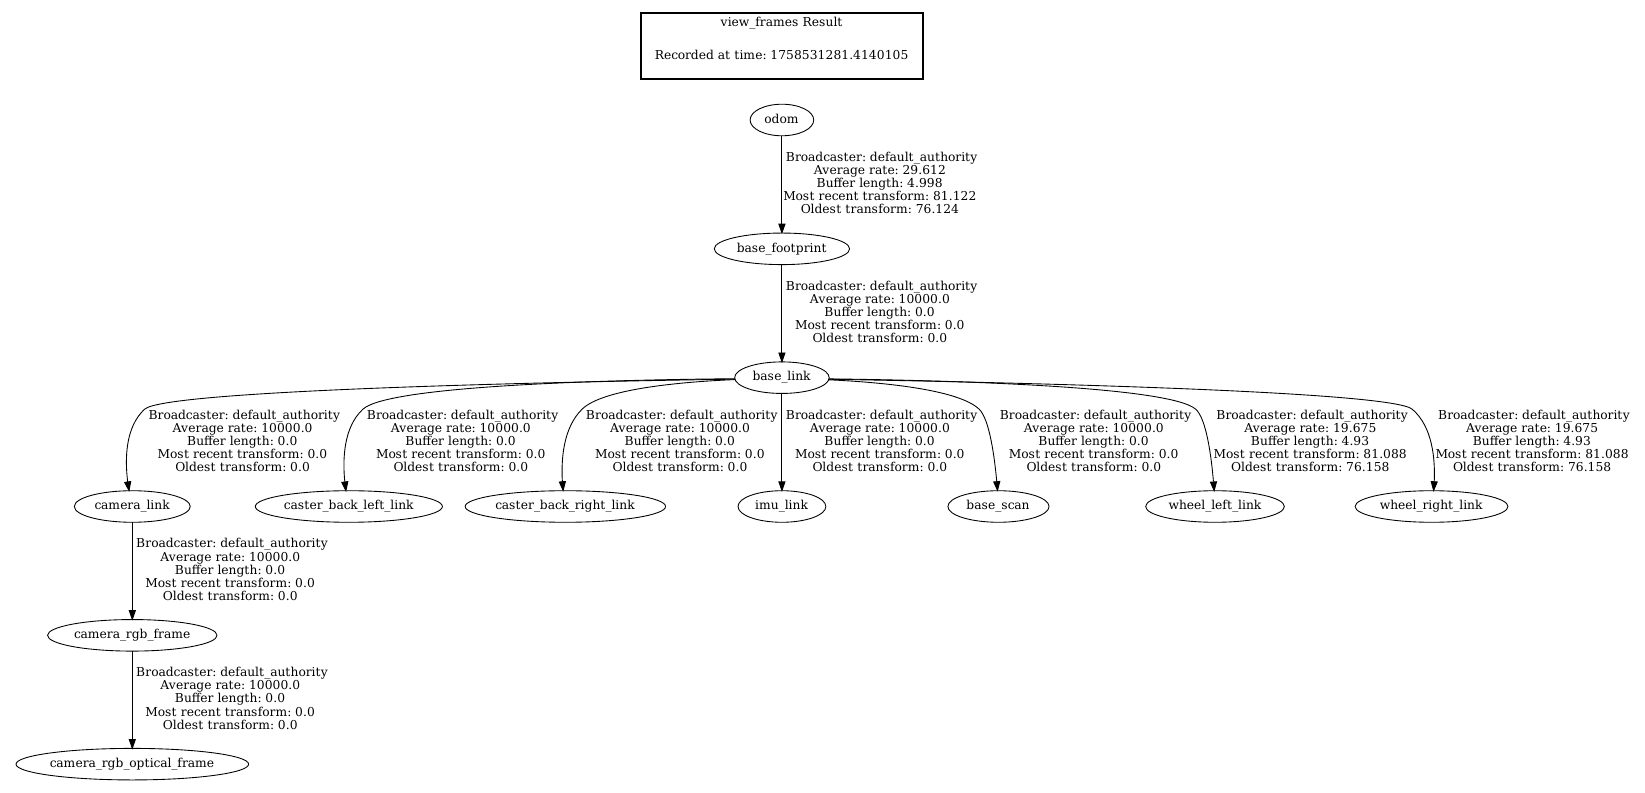
\includegraphics[width=1\textwidth]{tf_tree.png}
  \caption{Contoh TF Tree}
\end{figure}


% Module 2
\section{Modul 2: Mapping dengan RTAB-Map}

\subsection{SLAM dan RTAB-Map}
SLAM (Simultaneous Localization and Mapping) adalah proses di mana robot membangun peta lingkungan sambil menentukan posisinya di dalam peta tersebut. Pada dasarnya, SLAM dibagi menjadi dua yaitu map based SLAM dan graph based SLAM. Perbedaan paling mendasar adalah pada bagian lokalisasinya. Pada map based SLAM, lokalisasi dilakukan dengan melakukan registrasi data sensor ke map yang telah dibangun sebelumnya. Sedangkan pada graph based SLAM, lokalisasi dilakukan dengan registrasi sensor ke setiap graph yang dibangun sebelumnya.
\par
RTAB-Map (Real-Time Appearance-Based Mapping) adalah sebuah algoritma graph based SLAM yang menggunakan data visual (gambar) dan data jarak (misalnya dari LIDAR atau depth camera) untuk membangun peta 3D dari lingkungan sekitar. RTAB-Map dapat digunakan untuk berbagai aplikasi robotika, termasuk navigasi, inspeksi, dan pemetaan lingkungan. Untuk memperjelas bagaimana cara kerja Graph Based SLAM, silahkan simak video berikut: \href{https://youtu.be/saVZtgPyyJQ?si=qHGGJnJUz-iB19UF}{\textbf{Graph Based SLAM Explanation}}.

\subsection{RTAB-Map}
Kunci dari Graph Based SLAM adalah deteksi loop closure. Di RTAB-Map, deteksi loop closure menggunakan kamera. Algoritma dasar yang perlu dipelajari untuk mencari loop closure menggunakan kamera adalah Image Registration. Image Registration adalah proses mencocokkan dua gambar yang diambil dari sudut pandang yang berbeda untuk menemukan transformasi geometris antara keduanya. Contoh contoh algoritma yang sering dipakai adalah GFTT, FAST, BRIEF, ORB, SIFT, dan lain lain.
\newline
\textbf{RTAB-Map bukanlah Ready to Use SLAM, perlu dilakukan penyesuaian pada robot yang akan digunakan!}

\subsection{Penyesuaian RTAB-Map}
\subsubsection{Penyesuaian Sensor}
Di RTAB-Map, bisa menggunakan beberapa sensor, cara setting nya lewat parameter:
\begin{itemize}
  \item \textbf{subscribe\_depth}: Untuk kamera depth seperti realsense
  \item \textbf{subscribe\_scan}: Untuk LIDAR 2d
  \item \textbf{subscribe\_scan\_cloud}: Untuk LIDAR 3d
  \item \textbf{subscribe\_rgbd}: Untuk kamera RGBD seperti Kinect
  \item \textbf{subscribe\_stereo}: Untuk kamera stereo seperti Zed
  \item \textbf{subscribe\_odom}: Untuk odometri hardware atau sumber odometry lainnya
\end{itemize}
Jika sistem robot tidak memiliki source odometry, odometry bisa dihitung dari visual odometry atau icp odometry bawaan RTAB-Map. Untuk menggunakannya bisa menajalankan node lain yaitu \texttt{rgbd\_odometry} atau \textit{icp\_odometry}.

\subsubsection{Penyesuaian Loop Closure Detection}
Ada beberapa hal penting yang perlu diperhatikan dalam penyesuaian loop closure detection:
\begin{itemize}
  \item \textbf{Kp/DetectorStrategy}: Memilih algoritma image matching yang sesuai dengan kondisi lingkungan dan jenis kamera yang digunakan.
  \item \textbf{Kp/MaxFeatures}: Berapa banyak maksimal fitur (words) yang bisa disimpan dalam database. Perhatikan juga setiap algoritma akan menghasilkan jumlah fitur yang berbeda beda.
  \item \textbf{Vis/MinInliers}: Hasil dari scan matching juga berupa inliers yang telah diperoleh dari RANSAC. Semakin besar nilai inliers, semakin baik hasil scan matching. Namun, jika terlalu besar, bisa jadi tidak ada loop closure yang terdeteksi.
\end{itemize}

\subsubsection{Penyesuaian Graph Optimization}
Graph optimization adalah proses memperbaiki posisi node pada graph berdasarkan loop closure yang terdeteksi. Ada beberapa parameter penting yang perlu diperhatikan:
\begin{itemize}
  \item \textbf{Reg/Strategy}: Memilih mau menggunakan sensor apa untuk menghitung constraint per node pada graphnya. Bisa menggunakan icp atau visual atau gabungan keduanya. ICP dari LIDAR sedangkan visual dari kamera.
  \item \textbf{Optimizer/Strategy}: Memilih algoritma optimizer yang diinginkan (default GTSAM).
  \item \textbf{Optimizer/Iterations}: Semakin besar maka semakin lama iterasi optimasinya, hasilnya belum tentu lebih baik. Gunakan default saja jika tidak ada masalah.
  \item \textbf{RGBD/OptimizeMaxError}: Gerbang terakhir untuk optimasi, Jika hasil error nya terlalu besar maka loop closure akan di-reject dan graph tidak akan dioptimasi.
  \item \textbf{RGBD/OptimizeFromGraphEnd}: Ketika loop closure diterima, ada dua pendekatan optimasi, optimasi seluruh graph atau hanya dari node terakhir. Jika optimiasi dari seluruh graph, pasti akan membuat map atau estimasi pose robot loncat.
\end{itemize}

\subsubsection{Parameter Penting Lainnya}
\begin{itemize}
  \item \textbf{Mem/IncrementalMemory}: Dipastikan false, agar database dalam keadaan frozen saat pertama kali dihidupkan. Intinya, keadaan default adalah keadaan lokalisasi, bukan mapping. Jika ingin mapping, harus diaktifkan dengan service.
  \item \textbf{Mem/STMSize}: Berapa banyak node terakhir yang akan disimpan di Short Term Memory (STM). Node-node ini akan dibandingkan dengan node baru untuk mencari loop closure. Jika robot bergerak cepat, maka STM size harus lebih besar.
  \item \textbf{Mem/NotLinkedNodesKept}: Berapa banyak node yang tidak terhubung dengan loop closure yang akan disimpan di memori. Setting ini ke True agar databse tidak crash.
  \item \textbf{RGBD/NeighborLinkRefining}: Jika TF sensor sudah dipastikan bagus, maka parameter ini bisa diset True. Jika kurang percaya dengan hasil sensor, dan ingin lebih percaya dengan odometry, maka bisa diset False.
\end{itemize}

\subsubsection{Grid Map}
Grid hasil dari RTAB-Map berupa occupancy grid. Hasil dari occupancy grid ini tidak penting untuk lokalisasi karena RTAB-Map merupakan graph based SLAM. Biasanya, grid map ini digunakan untuk navigasi yang nantinya berupa global costmap. Ada beberapa parameter penting yang perlu diperhatikan:
\begin{itemize}
  \item \textbf{Grid/Sensor}: Jenis sensor yang digunakan untuk membuat grid. Bisa menggunakan laser scan, depth image, atau point cloud. Pilih sesuai dengan sensor yang dimiliki robot.
  \item \textbf{Grid/RangeMax}: Jarak maksimal dari sensor yang akan dimasukkan ke dalam grid. Jika jarak sensor lebih dari nilai ini, maka data tersebut akan diabaikan.
  \item \textbf{Grid/CellSize}: Ukuran sel grid. Semakin kecil ukuran sel, semakin detail peta yang dihasilkan, namun juga semakin besar ukuran peta dan semakin lama waktu pemrosesan.
\end{itemize}

\section{Module 3: Navigation with Nav2}
\subsection{planner\_server}
Planner server bertanggung jawab untuk merencanakan jalur dari posisi awal ke tujuan. Planner server menggunakan algoritma perencanaan jalur seperti A* atau Dijkstra untuk menemukan jalur terpendek yang menghindari obstacle. Planner server menerima permintaan perencanaan jalur dari client (misalnya, \texttt{nav2\_bt\_navigator}) dan mengembalikan jalur yang direncanakan dalam bentuk serangkaian pose (waypoints) yang harus diikuti oleh robot.
\subsubsection*{Parameter Penting planner\_server}
Beberapa parameter penting pada \texttt{planner\_server} yang perlu diperhatikan:
\begin{itemize}
  \item \textbf{use\_sim\_time}: Pilih \texttt{true} untuk simulasi, \texttt{false} untuk real time.
  \item \textbf{expected\_update\_rate}: Frekuensi update perencanaan jalur (dalam Hz).
  \item \textbf{planner\_plugin}: Plugin planner yang digunakan untuk perencanaan jalur.
\end{itemize}

\subsubsection*{Plugin Planner pada planner\_server}
\begin{table}[H]
  \centering
  \renewcommand{\arraystretch}{1.2}
  \begin{tabular}{|p{3cm}|p{8cm}|}
    \hline
    \textbf{Plugin}            & \textbf{Deskripsi dan Penggunaan}                                                                                                                                         \\
    \hline
    NavFn Planner              & Algoritma grid-based (Dijkstra/A*) untuk jalur terpendek. Cocok untuk omni, mecanum, dan differential drive robot.                                                        \\
    \hline
    Smac 2D Planner            & Grid-based A* dengan cost-awareness. Implementasi modern, cocok untuk omni, mecanum, dan differential drive robot.                                                        \\
    \hline
    Smac Hybrid-A* Planner     & Mempertimbangkan heading robot pada tiap node, menghasilkan path yang lebih realistis secara kinematik. Cocok untuk car-like robot (non-holonomic) dan ackerman steering. \\
    \hline
    Smac State Lattice Planner & Planner berbasis State Lattice dengan motion primitives precomputed (offline). Cocok untuk car-like robot (non-holonomic) dan ackerman steering.                          \\
    \hline
    Theta* Planner             & Algoritma Theta*, variasi A* yang memungkinkan any-angle paths (tidak terbatas pada grid horizontal/vertikal). Cocok untuk omni, mecanum, dan differential drive robot.   \\
    \hline
  \end{tabular}
  \caption{Plugin Planner pada planner\_server Nav2}
\end{table}

\subsection{controller\_server}
\texttt{Controller\_Server} bertanggung jawab untuk mengendalikan gerakan robot agar mengikuti jalur yang telah direncanakan oleh \texttt{planner\_server}. \texttt{controller\_server} menerima jalur (path) dari \texttt{planner\_server} dan menghasilkan perintah kecepatan (velocity commands) yang akan dikirim ke robot untuk mengikuti jalur tersebut.
\subsubsection*{Parameter Penting controller\_server}

Beberapa parameter penting pada \texttt{controller\_server} yang perlu diperhatikan:
\begin{itemize}
  \item \textbf{use\_sim\_time}: Pilih \texttt{true} untuk simulasi, \texttt{false} untuk real time.
  \item \textbf{controller\_frequency}: Frekuensi kontrol (dalam Hz).
  \item \textbf{odom\_topic}: Topik odometri yang digunakan untuk mendapatkan informasi posisi dan kecepatan robot.
  \item \textbf{progress\_checker\_plugin}: Plugin yang digunakan untuk memeriksa kemajuan robot menuju tujuan.
  \item \textbf{goal\_checker\_plugins}: Plugin yang digunakan untuk memeriksa apakah robot telah mencapai tujuan.
  \item \textbf{controller\_plugins}: Plugin yang digunakan untuk mengendalikan gerakan robot mengikuti jalur.
\end{itemize}

\subsubsection*{Plugin Progress Checker pada controller\_server}
\begin{table}[H]
  \centering
  \renewcommand{\arraystretch}{1.2}
  \begin{tabular}{|p{4cm}|p{7cm}|}
    \hline
    \textbf{Plugin}       & \textbf{Deskripsi dan Penggunaan}                                                                                                                                                                    \\
    \hline
    SimpleProgressChecker & Cocok untuk sebagian besar robot dan lingkungan. Memantau apakah robot membuat kemajuan yang cukup menuju tujuan berdasarkan jarak yang ditempuh.                                                    \\
    \hline
    PoseProgressChecker   & Cocok untuk robot yang memerlukan kontrol orientasi yang presisi. Memantau kemajuan posisi dan orientasi, memastikan robot tidak hanya bergerak menuju tujuan tetapi juga berorientasi dengan benar. \\
    \hline
  \end{tabular}
  \caption{Plugin Progress Checker pada controller\_server Nav2}
\end{table}

\subsubsection*{Plugin Goal Checker pada controller\_server}
\begin{table}[H]
  \centering
  \renewcommand{\arraystretch}{1.2}
  \begin{tabular}{|p{4cm}|p{7cm}|}
    \hline
    \textbf{Plugin}     & \textbf{Deskripsi dan Penggunaan}                                                                                                                                                                           \\
    \hline
    SimpleGoalChecker   & Cocok untuk sebagian besar robot dan lingkungan. Memeriksa apakah robot berada dalam toleransi jarak dan orientasi tertentu dari tujuan.                                                                    \\
    \hline
    StoppedGoalChecker  & Cocok untuk robot yang perlu berhenti sepenuhnya di tujuan. Selain toleransi jarak dan orientasi, memeriksa apakah kecepatan linier dan angular robot berada di bawah ambang batas tertentu.                \\
    \hline
    PositionGoalChecker & Cocok untuk robot yang hanya perlu mencapai posisi tertentu tanpa persyaratan orientasi yang ketat. Memeriksa apakah robot berada dalam toleransi jarak tertentu dari posisi tujuan, mengabaikan orientasi. \\
    \hline
  \end{tabular}
  \caption{Plugin Goal Checker pada controller\_server Nav2}
\end{table}

\subsubsection*{Plugin Controller pada controller\_server}
\begin{table}[H]
  \centering
  \renewcommand{\arraystretch}{1.2}
  \begin{tabular}{|p{4cm}|p{7cm}|}
    \hline
    \textbf{Plugin}                   & \textbf{Deskripsi dan Penggunaan}                                                                                                                                                                                                           \\
    \hline
    DWBLocalPlanner                   & Cocok untuk robot differential drive di lingkungan dinamis. Menggunakan pendekatan dynamic window untuk menilai trajektori berdasarkan kinematika dan costmap lokal.                                                                        \\
    \hline
    Regulated Pure Pursuit Controller & Cocok untuk robot yang memerlukan pengikutan jalur yang halus dan akurat. Menggunakan titik lookahead pada jalur untuk menentukan perintah kemudi, dengan regulasi kecepatan linier berdasarkan kelengkungan jalur dan kedekatan rintangan. \\
    \hline
  \end{tabular}
  \caption{Plugin Controller pada controller\_server Nav2}
\end{table}

\subsection{recoveries\_server}
Recoveries server bertanggung jawab untuk menjalankan tindakan pemulihan (recovery behaviors) ketika robot gagal dalam perencanaan atau navigasi. Misalnya, jika robot terjebak atau tidak dapat menemukan jalur, maka recovery behaviors akan membantu robot keluar dari kondisi tersebut.

\subsubsection*{Parameter Penting recoveries\_server}
\begin{itemize}
  \item \textbf{use\_sim\_time}: Pilih \texttt{true} untuk simulasi, \texttt{false} untuk real time.
  \item \textbf{costmap\_topic}: Topik costmap yang digunakan untuk mendeteksi obstacle.
  \item \textbf{recovery\_plugins}: Daftar plugin recovery yang dapat digunakan.
\end{itemize}

\subsubsection*{Plugin Recovery pada recoveries\_server}
\begin{table}[H]
  \centering
  \renewcommand{\arraystretch}{1.2}
  \begin{tabular}{|p{3cm}|p{8cm}|}
    \hline
    \textbf{Plugin} & \textbf{Deskripsi dan Penggunaan}                                                                              \\
    \hline
    Spin Recovery   & Memutar robot di tempat untuk mencari jalur bebas obstacle.                                                    \\
    \hline
    Backup Recovery & Memundurkan robot sejauh jarak tertentu agar keluar dari deadlock.                                             \\
    \hline
    Wait Recovery   & Robot berhenti sejenak, berguna jika obstacle yang menghalangi bersifat sementara (misalnya orang lewat).      \\
    \hline
    Clear Costmap   & Menghapus data obstacle di costmap lokal/global agar perencanaan jalur bisa diperbarui dengan kondisi terkini. \\
    \hline
  \end{tabular}
  \caption{Plugin Recovery pada recoveries\_server Nav2}
\end{table}

\subsection{bt\_navigator}
Behavior Tree (BT) Navigator adalah komponen utama yang mengatur alur navigasi menggunakan \textit{behavior tree}. BT memungkinkan fleksibilitas dan modularitas dalam mendefinisikan urutan aksi, percabangan, serta kondisi navigasi.

\subsection{global\_costmap}
Global costmap bertugas membuat representasi peta statis dan dinamis yang digunakan oleh global planner untuk merencanakan jalur dari posisi awal ke tujuan. Global costmap biasanya mencakup area besar, sehingga mampu melihat keseluruhan lingkungan.

\subsubsection*{Parameter Penting global\_costmap}
\begin{itemize}
  \item \textbf{global\_frame}: Frame referensi global, biasanya \texttt{map}.
  \item \textbf{robot\_base\_frame}: Frame dasar robot, biasanya \texttt{base\_link}.
  \item \textbf{update\_frequency}: Frekuensi update data costmap (Hz).
  \item \textbf{resolution}: Resolusi grid (m/cell). Semakin kecil nilainya, semakin detail tetapi lebih berat komputasinya.
  \item \textbf{robot\_radius}: Radius robot (m) yang digunakan untuk inflasi obstacle.
  \item \textbf{plugins}: Layer yang digunakan, biasanya:
        \begin{itemize}
          \item Static Layer: Mengambil data peta statis (dari SLAM/Map server).
          \item Obstacle Layer: Menggunakan sensor (Lidar/sonar).
          \item Inflation Layer: Memberikan jarak aman dari obstacle.
        \end{itemize}
\end{itemize}

\subsubsection*{Batasan Tuning global\_costmap}
\begin{itemize}
  \item \textbf{resolution}: Jangan terlalu kecil ($<0.02$ m/cell) karena memori dan CPU bisa overload.
  \item \textbf{width/height}: Sesuaikan dengan ukuran map (misalnya 50x50 m). Terlalu besar akan membuat costmap berat.
  \item \textbf{robot\_radius vs. inflation\_radius}: Jika \texttt{inflation\_radius < robot\_radius}, robot bisa menabrak obstacle. Jika terlalu besar ($>3 \times$ ukuran robot), jalur bisa tidak ditemukan.
\end{itemize}

\subsection{local\_costmap}
Local costmap digunakan oleh local planner (controller server) untuk menghindari obstacle secara dinamis. Local costmap biasanya rolling window yang mengikuti pergerakan robot, dengan area yang relatif kecil.

\subsubsection*{Parameter Penting local\_costmap}
\begin{itemize}
  \item \textbf{global\_frame}: Biasanya \texttt{odom}, karena hanya lokal dan tidak perlu akurat ke peta global.
  \item \textbf{robot\_base\_frame}: Frame dasar robot, biasanya \texttt{base\_link}.
  \item \textbf{rolling\_window}: Harus \texttt{true}, agar peta mengikuti robot.
  \item \textbf{width/height}: Lebar dan tinggi window (misalnya 6x6 m).
  \item \textbf{resolution}: Grid size (misalnya 0.05 m).
  \item \textbf{plugins}:
        \begin{itemize}
          \item Obstacle Layer: Membaca sensor (lidar, sonar, bumper).
          \item Inflation Layer: Menjaga jarak aman.
        \end{itemize}
\end{itemize}

\subsubsection*{Batasan Tuning local\_costmap}
\begin{itemize}
  \item \textbf{width/height}: Jangan terlalu besar ($>10$ m), karena costmap lokal menjadi lambat diproses.
  \item \textbf{robot\_radius}: Sesuaikan dengan dimensi robot sebenarnya. Jika terlalu besar, robot akan menganggap semua jalur sempit tidak bisa dilewati.
  \item \textbf{inflation\_radius}: Umumnya antara $1.2 \times$ sampai $2 \times$ \texttt{robot\_radius}. Jika terlalu kecil, robot bisa terlalu dekat dengan obstacle; jika terlalu besar, robot bisa gagal menemukan jalur.
  \item \textbf{update\_frequency}: Disarankan $5$–$10$ Hz. Terlalu tinggi bisa membebani CPU, terlalu rendah membuat respon robot lambat.
\end{itemize}

\end{document}
